\documentclass{article}
\usepackage{amsmath,amssymb,kotex,tabu,graphicx}
\usepackage[skipabove=10pt,innertopmargin=10pt,nobreak=true]{mdframed}
\usepackage{multicol}
\setlength{\columnseprule}{0.4pt}
\usepackage[margin=0.5in]{geometry}
\usepackage[symbol]{footmisc}
\renewcommand{\thefootnote}{\fnsymbol{footnote}}
\setlength{\skip\footins}{2cm}
\usepackage[inline]{enumitem}
\setenumerate{label=(\arabic*)}


\newcounter{num}
\newcommand{\theo}[1]
{\bigskip\bigskip\noindent\refstepcounter{num}\textbf{정리 \arabic{num})} #1\par\noindent}
\newcommand{\prob}[1]
{\bigskip\bigskip\noindent\refstepcounter{num}\textbf{문제 \arabic{num})} #1\par\noindent}
\newcommand{\exam}[1]
{\bigskip\bigskip\noindent\refstepcounter{num}\textbf{예시 \arabic{num})} #1\par\noindent}
\newcommand{\proo}
{\bigskip\noindent\textsf{증명)}}

\newcounter{anum}
\newcommand{\an}
{\bigskip\bigskip\noindent\refstepcounter{anum}\textbf{답 \arabic{anum})}\par\par\noindent}
\newcommand{\ann}
{\bigskip\bigskip\noindent\refstepcounter{anum}\textbf{답 \arabic{anum})}\quad}

\newcommand{\pb}[1]%\Phantom + fBox
{\fbox{\phantom{\ensuremath{#1}}}}

%\renewcommand{\arraystretch}{1.5}

\newcommand{\procedure}[1]{\begin{mdframed}\vspace{#1\textheight}\end{mdframed}}

\newcommand\ov[1]{\ensuremath{\overline{#1}}}
\newcommand\ovv[2]{\ensuremath{\overline{#1#2}}}
\newcommand{\cb}{\vfill\null\columnbreak}

\renewcommand{\baselinestretch}{1.5}

%%% Title
\title{성현 - 제곱근과 절댓값}
\date{\today}
\author{}

\begin{document}
\maketitle

\begin{multicols}{2}

%
\prob{다음을 계산하여라.}
\begin{enumerate}
\item
\(|6|\)
\item
\(|-3|\)
\item
\(|0|\)
\item
\(|-10|\)
\item
\(\sqrt{6^2}\)
\item
\(\sqrt{(-3)^2}\)
\item
\(\sqrt{0^2}\)
\item
\(\sqrt{(-10)^2}\)
\item
\(\sqrt{6}^2\)
\item
\(\sqrt{-3}^2\)
\item
\(\sqrt{0}^2\)
\item
\(\sqrt{-10}^2\)
\end{enumerate}
\cb

%
\theo{\(a\)가 실수일 때,}
\begin{enumerate}
\item
\(|a|=\begin{cases}a&(a\ge0)\\-a&(a\le0)\end{cases}\)
\item
\(\sqrt{a^2}=\begin{cases}a&(a\ge0)\\-a&(a\le0)\end{cases}\)
\item
\(\sqrt{a^2}=|a|\)
\item
\(\sqrt a^2=\begin{cases}a&(a\ge0)\\\text{답을 정할 수 없다.\footnotemark}&(a<0)\end{cases}\)
\end{enumerate}
\footnotetext{고등학교 1학년 과정에서는 \(i=\sqrt{-1}\)을 도입한다.
이 숫자 \(i\)는 \(i^2=-1\)을 만족시키는 새로운 수이다.
\(i\)를 가지고 문제 1)의 (10), (12)를 계산하면
%그러면 
\begin{align*}
(10)\;\;&\;\;\sqrt{-3}^2=(\sqrt 3\sqrt{-1})^2=\sqrt3^2i^2=3\cdot (-1)=-3\\
(12)\;\;&\;\;\sqrt{-10}^2=(\sqrt{10}\sqrt{-1})^2=\sqrt{10}^2i^2=10\cdot (-1)=-10
\end{align*}
이다.}


%
\exam{다음 문장들 중 옳은 것에는 `O', 틀린 것에는 `X' 표시를 하여라.
틀린 문장은 왜 틀렸는지 예를 들어 설명하여라.
}
\begin{enumerate}
\item
\(x\)가 실수이면 \(\sqrt{(x-1)^2}=|x-1|\)이다.
\dotfill[O]
\item
\(y\)가 실수이면 \(\sqrt{y^2}=y\)이다.
\dotfill[X, \(y=-2\)]
\item
\(t\le0\)이면 \(\sqrt t^2\neq t\)이다.
\dotfill[X, \(t=0\)]
\end{enumerate}
\cb

%
\prob{다음 문장들 중 옳은 것에는 `O', 틀린 것에는 `X' 표시를 하여라.
틀린 문장은 왜 틀렸는지 예를 들어 설명하여라.
}
\begin{enumerate}
\item
\(b>2\)일 때, \(\sqrt{(b-2)^2}=b-2\)이다.
\dotfill[\qquad\qquad]
\item
\(b>0\)일 때, \(\sqrt{(b-2)^2}=b-2\)이다.
\dotfill[\qquad\qquad]
\item
\(n\)이 자연수이면 \(\sqrt n^2=n\)이다.
\dotfill[\qquad\qquad]
\item
\(k\)가 자연수이면 \(\sqrt{k^2}=-k\)이다.
\dotfill[\qquad\qquad]
\item
\(c<-4\)일 때, \(\sqrt{(c+4)^2}=-c-4\)이다.
\dotfill[\qquad\qquad]
\item
\(x\)가 실수일 때, \(|-x|=|x|\)이다.
\dotfill[\qquad\qquad]
\item
\(x\)가 실수일 때, \(\sqrt{(-x)^2}=\sqrt{x^2}\)이다.
\dotfill[\qquad\qquad]
\end{enumerate}

%
\exam{\(0\le a\le 3\)일 때, 다음을 계산하여라.}
\begin{enumerate}\label{prev_exam}
\item
\(|a-3|+|a|=|a-3|+|a|=-(a-3)+a=3\)
\item
\(2|a-3|+3|a|=2\{-(a-3)\}+3a=a+6\)
\item
\(\sqrt{(a-5)^2}-|a+2|=|a-5|+|a+2|=-(a-5)-(a+2)=-2a+3\)
\end{enumerate}


%
\prob{\(2\le b\le 4\)일 때, 다음을 계산하여라.}
\begin{enumerate}\label{prev_prob}
\item
\(|b-2|+|b-4|=\)
\item
\(2|b-2|-3|b-4|=\)
\item
\(|2-b|-|b-4|=\)
\item
\(|b|+|-b|=\)
\item
\(\sqrt{(b-2)^2}-\sqrt{(b-4)^2}=\)
\end{enumerate}

%
\prob{\(-1<c<1\)일 때, 다음을 계산하여라.}
\begin{enumerate}
\item
\(\sqrt{(c-1)^2}+\sqrt{(c+1)^2}=\)
\item
\(3|c-1|+4|c+1|=\)
\item
\(|c-2|+3|c+2|\)
\item
\(\sqrt{(4-c)^2}+\sqrt{(-1-c)^2}\)
\end{enumerate}
%
%\theo{\(a\ge0\)일 때}
%\[\sqrt a^2=a=\begin{cases}a&(a\ge0)\\\text{생각하지 않는다.}&(a<0)\end{cases}\]

%
\prob{다음을 계산하여라.}
\begin{enumerate}
\item
\(|5-1|\)
\item
\(|4-(-3)|\)
\item
\(|2-4|\)
\item
\(|4|\)
\end{enumerate}

%
\prob{아래와 같은 수직선에 대하여 다음을 계산하여라.}
\begin{center}
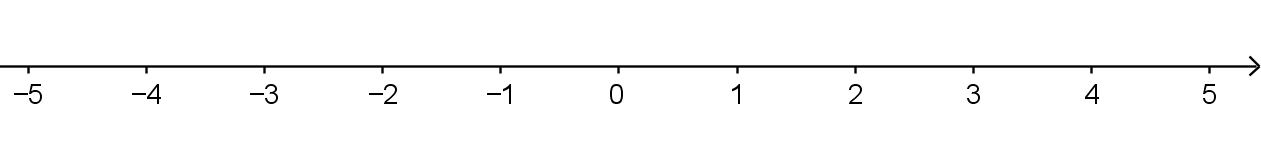
\includegraphics[width=\columnwidth]{x_pm5}
\end{center}
\begin{enumerate}
\item
5와 1 사이의 거리
\item
4와 \(-3\) 사이의 거리
\item
2와 4 사이의 거리
\item
4와 0 사이의 거리
\end{enumerate}

%
\theo{실수 \(a\), \(b\)에 대하여}
\[|a-b|=\text{수직선 위의 \(a\)와 \(b\) 사이의 거리}\]
이다.

%
\exam{다음은 예시 \ref{prev_exam})의 (1)를 다시 계산하는 과정이다. 빈칸을 채워라.}
\begin{center}
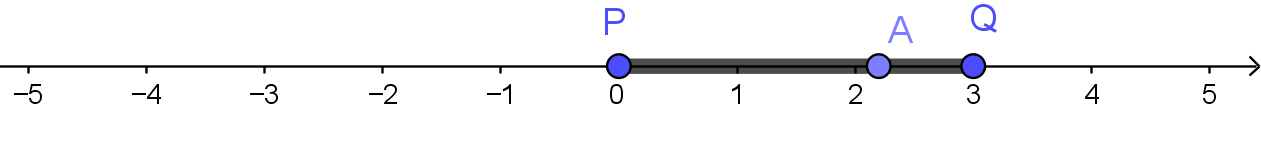
\includegraphics[width=\columnwidth]{x_pm5_A}
\end{center}
0을 나타내는 점을 \(P\), 3을 나타내는 점을 \(Q\)라고 하자.
\(a\)를 나타내는 점을 \(A\)라고 하면 \(A\)는 \(P\)와 \(Q\) 사이를 움직인다.
\begin{align*}
|a-3|=\fbox{\ovv AQ}\\
|a|=\fbox{\ovv AP}
\end{align*}
이므로
\(|a-3|+|a|=\fbox{\ovv AQ}+\fbox{\ovv AP}\)이다.
\(P\)의 위치에 관계없이 \(\fbox{\ovv AQ}+\fbox{\ovv AP}=\fbox{\ovv PQ}\)이므로 
\[|a-3|+|a|=\fbox{\ovv AQ}+\fbox{\ovv AP}=\fbox{\ovv PQ}=3\]
\cb

%
\prob{다음은 예시 \ref{prev_prob})의 (1)를 다시 계산하는 과정이다. 빈칸을 채워라.}
\begin{center}
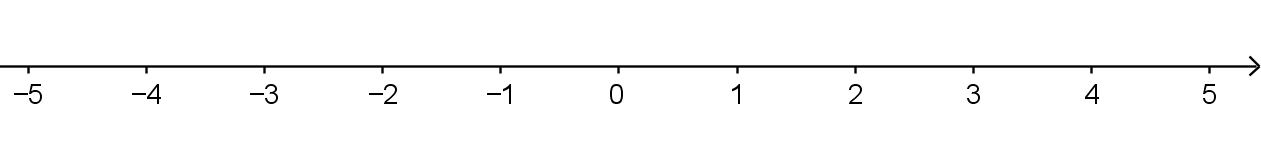
\includegraphics[width=\columnwidth]{x_pm5}
\end{center}
2를 나타내는 점을 \(P\), 4를 나타내는 점을 \(Q\)라고 하자.
\(b\)를 나타내는 점을 \(B\)라고 하면 \(B\)는 \(P\)와 \(Q\) 사이를 움직인다.
\begin{align*}
|b-2|=\pb{\ovv AQ}\\
|b-4|=\pb{\ovv AP}
\end{align*}
이므로
\(|b-2|+|b-4|=\pb{\ovv AQ}+\pb{\ovv AP}\)이다.
\(P\)의 위치에 관계없이 \(\pb{\ovv AQ}+\pb{\ovv AP}=\pb{\ovv PQ}\)이므로 
\[|b-2|+|b-4|=\pb{\ovv AQ}+\pb{\ovv AP}=\pb{\ovv PQ}=2\]

%
\prob{\(1<x<y<4\)일때,}
\[|1-x|+|x-y|+|y-4|\]
의 값을 구하여라.
\cb

%
\an
\begin{enumerate*}
\item6
\item3
\item0
\item10\\
\item6
\item3
\item0
\item10\\
\item6
\item 답을 정할 수 없다.\\
\item0
\item 답을 정할 수 없다.\\
\end{enumerate*}

\stepcounter{anum}\stepcounter{anum}

%
\ann
\begin{enumerate*}
\item O
\item X
\item O
\item X
\item O
\item O
\item O
\end{enumerate*}
\stepcounter{anum}

%
\ann
\begin{enumerate*}
\item $2$
\item $5b-16$
\item $2b-6$
\item $2b$
\item $2b-6$
\end{enumerate*}

%
\ann
\begin{enumerate*}
\item $2$
\item $c+7$
\item $2c+8$
\item $5$
\end{enumerate*}

%
\ann
\begin{enumerate*}
\item 4
\item 7
\item 2
\item 4
\end{enumerate*}

%
\ann
\begin{enumerate*}
\item 4
\item 7
\item 2
\item 4
\end{enumerate*}

\stepcounter{anum}\stepcounter{anum}
%
\an
\begin{center}
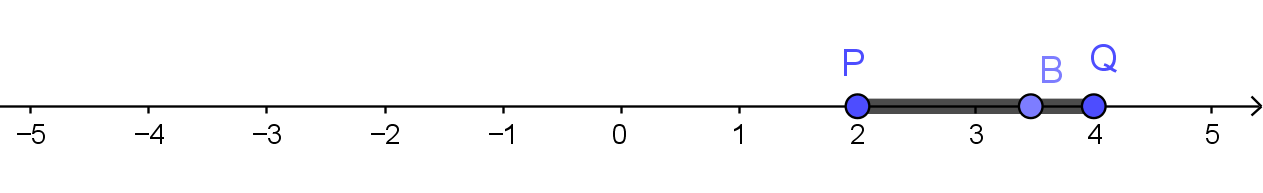
\includegraphics[width=\columnwidth]{x_pm5_B}
\end{center}
2를 나타내는 점을 \(P\), 4를 나타내는 점을 \(Q\)라고 하자.
\(b\)를 나타내는 점을 \(B\)라고 하면 \(B\)는 \(P\)와 \(Q\) 사이를 움직인다.
\begin{align*}
|b-2|=\fbox{\ovv BP}\\
|b-4|=\fbox{\ovv BQ}
\end{align*}
이므로
\(|b-2|+|b-4|=\fbox{\ovv BP}+\fbox{\ovv BQ}\)이다.
\(P\)의 위치에 관계없이 \(\fbox{\ovv BP}+\fbox{\ovv BQ}=\fbox{\ovv PQ}\)이므로 
\[|b-2|+|b-4|=\fbox{\ovv BP}+\fbox{\ovv BQ}=\fbox{\ovv PQ}=2\]

%
\ann 3
\clearpage
\end{multicols}

\end{document}







